In this chapter, we discuss techniques to sample static properties of systems in thermodynamic equilibrium.
Our focus will be on the microcanonical and canonical ensembles, for which the corresponding sampling dynamics are described by the Hamiltonian and Langevin equations.
Consequently, the bulk of this chapter is dedicated to theoretical discussions of their properties, as well as the description of numerical integration strategies.

\section{Microcanonical averages}
We start by describing methods to sample microcanonical averages, first describing a few qualitative properties of Hamiltonian dynamics. 
These will serve as criteria to determine viable candidate numerical schemes, which will be required to preserve, either exactly or asymptotically,
those qualitative properties.
We then turn to the description of such structure-preserving schemes, and their energy conservation properties, concluding by a numerical illustration.

\subsection{Elementary properties of Hamiltonian dynamics}
The Hamiltonian dynamics \eqref{eq:hamiltonian_dynamics} rewrites in matrix form, with $X_t=(q_t,p_t)$:
\begin{equation}\label{eq:hamiltonian_dynamics_matrix_form} \text d X_t=J\nabla H(X_t)\,\dt,\end{equation}
where $J$ is the symplectic matrix

$$J = \begin{pmatrix}
    0_{dN} & \Id_{dN}\\ -\Id_{dN} & 0_{dN}.
\end{pmatrix}$$

Applying the chain rule to any smooth function $\varphi: \mathcal E \to \R$, we obtain
        $$ \text d \varphi(X_t)= \text d X_t^{\intercal} \nabla \varphi(X_t)=(J \nabla H(X_t))^\intercal \nabla \varphi(X_t)\dt=(\nabla_p H \cdot \nabla_q - \nabla_q H \cdot \nabla_p)\varphi(X_t)\dt$$
        This motivates the following.
        \begin{definition}[Generator of the Hamiltonian dynamics]
            We define the generator associated with the Hamiltonian dynamics to be the operator $\cL_{\text{H}}$ acting on smooth functions as
        \begin{equation}
            \label{eq:hamiltonian_generator}
            \cL_{\mathrm{ham}}\varphi=(\nabla_p H \cdot \nabla_q - \nabla_q H \cdot \nabla_p)\varphi=\left(J\nabla H\right)^\intercal \nabla \varphi.
        \end{equation}
    \end{definition}
    We can split the generator as the sum of two elementary operators,
    $$\cLham=A+B,$$
    with
    \begin{equation}
        \label{eq:Lham_splitting}
        A=\left(M^{-1}p\right)\cdot \nabla_q \qquad B=-\nabla V(q)\cdot \nabla_p.
    \end{equation}
    The generator allows us to quantify the rate of change of an observable $\varphi$ under the evolution of the system. If we define, for $t\geq 0$, the evolution operators 
    $$P_t \varphi (q_0,p_0) = \varphi(\Phi_t(q_0,p_0)),$$
where $\Phi$ is the flow associated with the Hamiltonian dynamics, that is the collection of maps $(\Phi_t)_{t\geq 0}$, defined by
    $\Phi_t (q_0,p_0) = (q_t,p_t)$, the unique solution to \eqref{eq:hamiltonian_dynamics} with initial conditions  $(q_0,p_0)$, then we formally have:

    $$ \frac \partial{\partial t} P_t \varphi (q,p)= \partial_t \varphi(q_t,p_t)= \cLham \varphi(q_t,p_t)=\cLham P_t \varphi(q,p)=P_t\cLham \varphi(q,p).$$
    
    In the following result, we collect certain qualitative properties of Hamiltonian dynamics.
    \begin{prop}[Properties of Hamiltonian dynamics]
        \label{prop:hamiltonian_properties}
        Assume that the Hamiltonian $H$ \eqref{eq:hamiltonian} is $C^2$ on~$\mathcal E$ and that the flow $\Phi_t$ is globally defined for $t\in\R$. Then the following properties hold.
        \begin{enumerate}[i)]
            \item Group structure: \[\forall\, t,s\in \R,\qquad \Phi_t \circ \Phi_s = \Phi_{t+s},\, \Phi_0=\Id.\]
            \item Energy preservation: \[\frac{\mathrm{d}H(q_t,p_t)}{\dt}=0.\]
            \item Conservation of the Lebesgue measure: \[\forall \,\text{Lebesgue-measurable}\,D\subseteq \mathcal{E},\,\forall t\geq 0,\qquad|\Phi_t(D)|=|D|.\]
            \item Symplecticity: \[\forall t\geq 0,\qquad\nabla \Phi_t^\intercal J \nabla \Phi_t = J.\]
            \item Time reversibility: \[\Phi_t \circ \cR \circ \Phi_t=\mathcal R.\]
        \end{enumerate}
        The notation $\nabla$ corresponds to \eqref{eq:jacobian}, and the map $\mathcal R$ is the momentum-reversing involution
        \[\mathcal R(q,p)=(q,-p).\]
    \end{prop}
    \begin{proof}[Hints of proof.]
        \begin{enumerate}[i)]
            \item This property expresses the fact that the Hamiltonian evolution is autonomous, and follows from uniqueness in the Cauchy--Lipschitz theorem. This allows one to formally interpret the flow as a group action of $\R$ on $\mathcal E$.
            \item The energy conservation property simply follows from applying $\cLham$ to $H$.
            \item This property, known as Liouville's theorem, holds generally for any divergent-free flow. Its proof is based on a time differentiation of the determinant $\det\left(\nabla \Phi_t\right)$, and observing that the Hamiltonian vector field is divergence free: \[\mathrm{div}\left(J\nabla H\right)=\mathrm{div}_q\left(\nabla_p H\right)-\mathrm{div}_p\left(\nabla_q H\right)=0.\]
            \item The property is trivially satisfied at time $t=0$. A straightforward calculation shows that the time derivative of the symplecticity condition for $\Phi_t$ is $0$, which proves the claim. Let us remark that this property also implies property iii), since it shows $\det(\nabla\Phi_t)^2\det(J)=\det(J) \implies |\det(\nabla\Phi_t)|=1$.
            \item This again follows by uniqueness of trajectories: by observing that, for a fixed initial condition $(q_0,p_0)$, a time differentiation of the trajectory $(q_{-t},-p_{-t})=\mathcal R\, \circ\, \Phi_{-t}(q_0,p_0)$  shows it is Hamiltonian. Thus it must coincide with $\Phi_t(q_0,-p_0)=\Phi_t \circ \mathcal R (q_0,p_0)$. This can be restated as an equality of mappings, $\mathcal R \circ \Phi_{-t}=\Phi_t \circ \mathcal R$. Precomposing by $\Phi_t$ on each side yields the result using property i).
        \end{enumerate}
    \end{proof}

    \begin{remark}
        \label{rem:non_separable_hamiltonian}
        Properties \textit{i)} to \textit{iv)} above are still valid for any dynamics of the form \eqref{eq:hamiltonian_dynamics_matrix_form}, thus it is possible to consider dynamics 
        with more general Hamiltonians, which still obey them, disregarding issues of well-posedness. Property \textit{v)}, however uses the additional
        property that the classical Hamiltonian is separable into a kinetic and potential part, and that the kinetic part is an even function of $p$.
    \end{remark}   

    Property \textit{ii)} in the proposition above asserts that Hamiltonian trajectories remain on the constant energy manifold $S(H(q_0,p_0))$ defined in \eqref{eq:constant_energy_manifold}.
    Since this is the support of the microcanonical measure $\mu_{\mathrm{mc,E}}$, it is natural to ask whether the Hamiltonian dynamics can be used to sample the microcanonical measure, by means of ergodic averages.
    A minimum requirement for this to hold is that the measure is left invariant under Hamiltonian evolution. This is indeed the case. Consider a Hamiltonian trajectory $(q_t,p_t)$ such that $H(q_0,p_0)=E$. For $g$ and $f$ test functions,

    \begin{align*}
        \int_{\R} g(E)\int_{\mathcal E}f(q_t,p_t)\,\mathrm{d}\mu_{\mathrm{mc,E}}(q,p)\,\mathrm{d}E&=\frac1{Z_{\mathrm{E}}}\int_{\mathcal E} g(H(q,p))\left(f\circ \Phi_t\right) (q,p)\,\mathrm{d}q\,\mathrm{d}p\\
        &=\frac1{Z_{\mathrm{E}}}\int_{\mathcal E} g(H\circ \Phi_{-t}(\tilde q,\tilde p))f (\tilde q,\tilde p)\,\mathrm{d}\tilde q\,\mathrm{d}\tilde p\\
        &=\frac1{Z_{\mathrm{E}}}\int_{\mathcal E} g(H(\tilde q,\tilde p))f(\tilde q,\tilde p)\,\mathrm{d}\tilde q\,\mathrm{d}\tilde p\\
        &=\int_{\R}g(E)\int_{\mathcal E}f(\tilde q,\tilde p)\,\mathrm{d}\mu_{\mathrm{mc,E}}(q,p)\,\mathrm{d}E.
    \end{align*}
    the absence of a Jacobian determinant term in the change of variables from the second to the third line follows from property iii) in Proposition \ref{prop:hamiltonian_properties}, while the passage from the second to the third line is justified by the energy conservation property.
    This shows that the microcanonical measure is invariant under the Hamiltonian dynamics, but it is easy to construct examples where ergodic averages fail to converge to the correct value, as the following simple example shows.

    \begin{example}[A non-ergodic system]\label{ex:non_ergodic_system}
        We consider the following one-dimensional system with $\mathcal E= \mathbb T \times \R$, and the potential given by 
        \[V(q)=\cos\left(4\pi\left[q-\frac12\right]\right).\]
        
        The constant-energy manifold $S(0)$ consists of two disjoint compact connected components (see Figure \ref{fig:non_ergodic_system}). The observable
        \[\varphi(q,p)=\1_{q>\frac12}-\1_{q<\frac12}\]
        is constant on each component of $S(0)$, and has zero average with respect to $\mu_{\mathrm{mc,0}}$ by symmetry, but ergodic averages do not converge, since 
        \[\frac{1}{T} \int_0^T \varphi(q_t,p_t)\mathrm{d}t =  \frac{1}{T}\int_0^T \varphi(q_0,p_0)\mathrm{d}t=\varphi(q_0,p_0)\,\in\{\pm 1\}.\]
        \begin{figure}[htbp]
            \begin{center}
              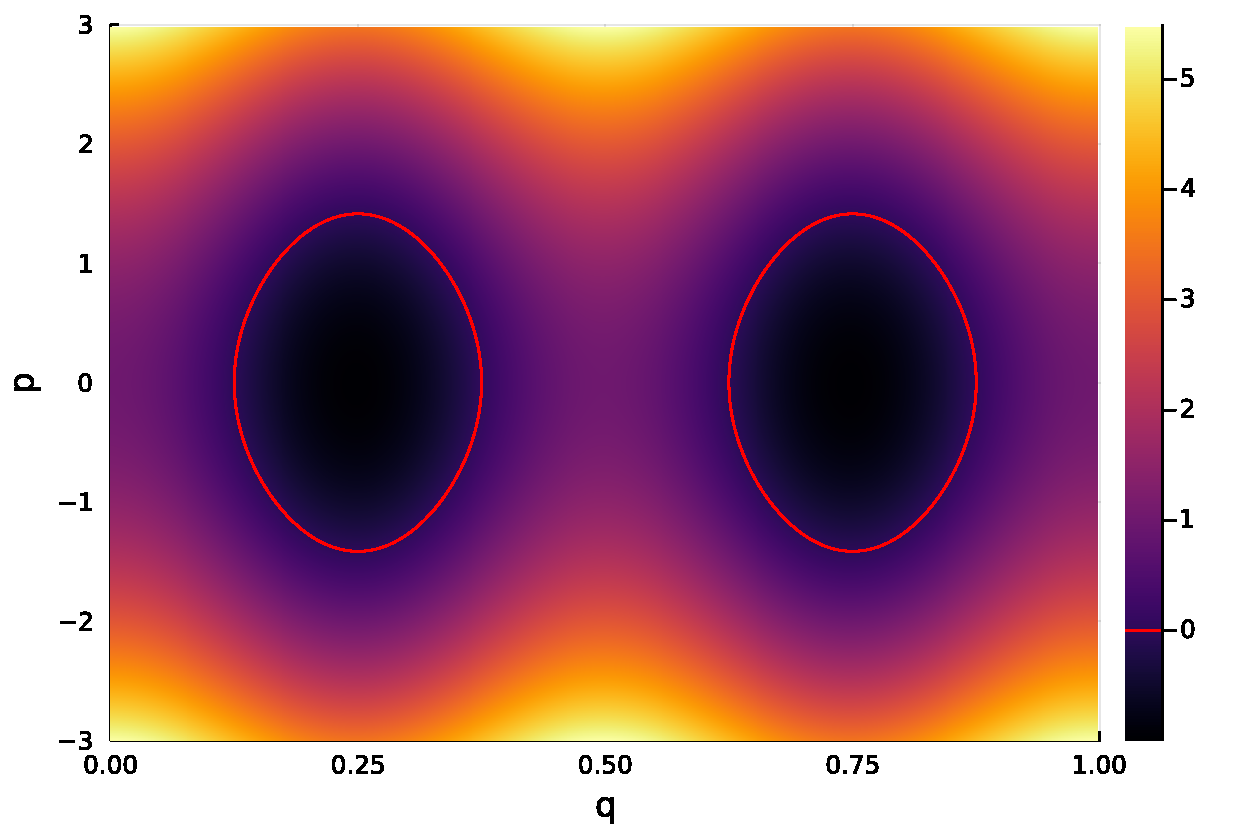
\includegraphics[width=0.7\linewidth]{figures/chapter1/ergodicity.pdf}
              \caption{ \label{fig:non_ergodic_system}
                The Hamiltonian landscape for the potential $V$ of Example \ref{ex:non_ergodic_system} , with $S(0)$ plotted in red.
              }
            \end{center}
          \end{figure}
    \end{example}

    The issue of ergodicity is in general very hard to tackle for realistic systems, and in practice is often taken as a working hypothesis.
     Besides, it may happen that for observables satisfying some symmetries in the constant energy manifold converge to the correct microcanonical average even in the absence of ergodicity.
     This is, for example, the case for the kinetic energy observable in our Example \ref{ex:non_ergodic_system}.

    \subsection{Numerical schemes for Hamiltonian dynamics}

    It not impossible, except for a restricted class of systems, which do not typically arise in practice, to analytically integrate Hamilton's equation \eqref{eq:hamiltonian_dynamics}. For this reason, one must resort to numerical schemes, which provide approximations of the flow map over one timestep.
    More precisely, for a fixed timestep $\Delta t$, if one has an approximation of the flow 
    \[\widetilde{\Phi}_{\Delta t}\approx\Phi_{\Delta t},\]
    one can deduce discrete approximations of the evolution by iteration:
    \begin{equation}\label{eq:discrete_dynamics}(q^n,p^n)\defeq \widetilde{\Phi}_{\Delta t}^n(q_0,p_0)\approx (q_{n\Delta t},p_{n\Delta t}),\end{equation}
    which can then be used as sample points for the computation of empirical averages, discrete counterparts to the ergodic averages \eqref{eq:ergodic_averages},
    \begin{equation}
        \label{eq:discrete_ergodic_averages}
        \frac 1N_{\mathrm{iter}}\sum_{k=0}^{N_{\mathrm{iter}}} \varphi(q^k,p^k).
    \end{equation}
    In most common applications involving ordinary differential equations, the aim is to approximate the exact solution as precisely as possible over a given domain.
    In the case of sampling trajectory averages in molecular dynamics, however, the time domain is usually very large, because simulating long trajectories is a requirement to ensure that a representative portion of phase space is explored. As a consequence, it is in practice impossible to obtain precise solutions over a long time at the level of trajectories, because the evolution's sensitivity to initial conditions will cause small initial errors to rapidly blowup. 
    Furthermore, one does not really \textit{care} about the exact evolution, since the dynamics are merely used as a sampling device. Instead, one key requirement is that the dynamics stay on or close to the constant energy manifold associated with a given initial condition. It can be shown through eigenanalysis that for simple linear systems, this requirement is not satisfied by standard ODE numerical methods such as the explicit and implicit Euler schemes, or the RK4 method, for which the energy may exponentially increase or decrease.
    This has the practical effect that for reasonably sized atomic systems, numerical instabilities render the simulations nonsensical after only a few time steps, which is far from what is needed to obtain good estimates.
    One must then devise dedicated numerical methods, guided by the aim to preserve qualitative properties of the Hamiltonian evolution. It turns out that splitting schemes, based on operator splitting approximations of the Hamiltonian evolution operator over one timestep, preserve crucial qualitative properties of the Hamiltonian evolution.

    An important observation is that if one considers each part of \eqref{eq:Lham_splitting} as a generator in its own right, the corresponding elmentary dynamics are analytically integrable.
    \begin{remark}
        \label{rem:Lham_splitting_semigroups}
        Consider the two dynamics defined by
        \begin{equation}
            \label{eq:Lham_splitting_dynamics_A}
            \left\{\begin{aligned}
                \dif q_t^A&=M^{-1}p_t^A\dif t,\\
                \dif p_t^A&=0,
            \end{aligned}\right.
        \end{equation}
        and
        \begin{equation}
            \label{eq:Lham_splitting_dynamics_B}
            \left\{\begin{aligned}
                \dif q_t^B&=0,\\
                \dif p_t^B&=-\nabla V(q_t^B)\dif t.
            \end{aligned}\right.
        \end{equation}
        These can be analytically solved as
        \begin{equation}
            \label{eq:Lham_splitting_dynamics_solved}
            \left\{\begin{aligned}
                &\left(q_t^A,p_t^A\right)=\left(q_0^A+tp_0^A,p_0^A\right),\\
                &\left(q_t^B,p_t^B\right)=\left(q_0^B,p_0^B-t\nabla V\left(q_0^B\right)\right).
            \end{aligned}\right.
        \end{equation} 
        Moreover, these evolutions are of Hamiltonian form, with Hamiltonians corresponding respectively to the kinetic part and the configurational part only, and have corresponding generators $A$ and $B$.
        We denote by $\left(\Phi^A_t\right)_{t \in \R}$ and $\left(\Phi^B_t\right)_{t\in\R}$ their respective flow maps.
    \end{remark}
    This observation suggests the following general recipes to construct a class of numerical schemes for the Hamiltonian dynamics, named splitting schemes. We consider approximations of the form
    \begin{equation}\label{eq:flow_splitting_approximation}\Phi_{\Delta t}\approx \Phi^{G_k}_{\Delta t_k}\circ \dotsm \circ \Phi^{G_1}_{\Delta t_1},\end{equation}
    where $G_i\in\{A,B\}$ for all $i$ and $\sum_{G_i=A}\Dt_i=\sum_{G_i=B}\Dt_i=1$. We will be considering three schemes, the simplest of which are the symplectic Euler schemes.
    The symplectic Euler schemes are defined by the following update equations:
    
    \begin{equation}\label{eq:symplectic_euler_A}
    \left\{\begin{aligned}
         p^{n+1} &=p^n -\nabla V(q^n)\Delta t,\\
         q^{n+1} &=q^n + M^{-1}p^{n+1}\Delta t,
    \end{aligned}\right.
    \end{equation}
    and
    \begin{equation}\label{eq:symplectic_euler_B}
        \left\{\begin{aligned}
             q^{n+1} &=q^n +M^{-1}p^n\Delta t,\\
             p^{n+1} &=p^n - \nabla V(q^{n+1})\Delta t.
        \end{aligned}\right.
    \end{equation}

    These correspond respectively to the splittings
    $\Phi_{\Delta t}^A\circ\Phi_{\Delta t}^B\defeq \Phi_{\Delta t}^{BA}$
    and
    $\Phi_{\Delta t}^B\circ\Phi_{\Delta t}^A\defeq \Phi_{\Delta t}^{AB}$.
    The velocity Verlet scheme is based on the symmetric splitting
    $\Phi_{\Delta t/2}^B\circ\Phi_{\Delta t}^A\circ\Phi_{\Delta t/2}^B\defeq \Phi_{\Delta t}^{BAB}$,
    Its update equation is given by
    \begin{equation}\label{eq:verlet}
        \left\{\begin{aligned}
             p^{n+\frac12} &=p^n - \frac{\Delta t}{2}\nabla V(q^n)\\
             q^{n+1} &=q^n + \Delta t M^{-1}p^{n+\frac 12}\\
             p^{n+1} &= p^{n+\frac12}-\frac{\Delta t}{2}\nabla V(q^{n+1}).
        \end{aligned}\right.
    \end{equation}
    We have announced above that these numerical schemes preserve some qualitative properties of the Hamiltonian dynamics. We now turn to making this statement precise.
    Let us fix an evolution operator $\tilde\Phi_{\Delta t}$ corresponding to a splitting of the form \eqref{eq:flow_splitting_approximation} with a timestep $\Dt>0$.
    Recall the properties in \ref{prop:hamiltonian_properties}. Then analogous properties can be stated for each of the schemes. We will refer to these analogous using the same names and indexing, but where $\Phi_t$ is replaced by $\tilde\Phi_{\Delta t}$ regardless of $t$.
    We further say a splitting is \textit{symmetric} if the corresponding order of operators $A$ and $B$ is a palindrome. The velocity Verlet splitting is symmetric, while the symplectic Euler splittings are not.
    We may then go through the properties in Proposition \ref{prop:hamiltonian_properties}, listing those which apply, and those which have to be modified.
        \begin{enumerate}[i)]
            \item Group structure: the analogous statement is a group action of $\mathbb{Z}$ on $\mathcal E$. This holds if the splitting is symmetric: then, $\tilde\Phi_{\Dt}^{-1}=\tilde\Phi_{-\Dt}$.
            \item Energy preservation: this does not hold as is, but does in a weakened sense that we discuss below.
            \item Conservation of the Lebesgue measure: this holds for all splittings.
            \item Symplecticity: similarly, this holds for all splittings.
            \item Time-reversibility: this holds for all symmetric splittings.
        \end{enumerate}
    \begin{proof}[Hints of proofs]
        For every one of these properties, the strategy is the same. From Proposition \ref{prop:hamiltonian_properties}, each one of them holds for $\Phi_{\Dt}^A$ and for $\Phi_{\Dt}^B$.
        The aim is then to show that these properties are stable, at best under composition, and at worst under symmetric composition.
        \begin{enumerate}[i)]
            \item This simply follows from writing \[\left(g_1 \circ g_2 \circ \dotsm \circ g_2\circ g_1\right)^{-1}=g_1^{-1}\circ g_2^{-1}\circ \dotsm \circ g_2^{-1}\circ g_1^{-1},\] and using property \textit{i)} applied to $\Phi_{\Dt}^A$ and $\Phi_{\Dt}^B$.
            \item This is a crucial and slightly subtle point, to which we return in more detail below.
            \item This follows trivially by composition (or alternatively by symplecticity). For any measure preserving measurable maps $f$ and $g$, \[|f \circ g(D)|=|g(D)|=|D|.\] 
            \item This follows from the fact that any composition of symplectic maps is symplectic. This, in turn, follows from the multivariate chain rule below, and applying the symplectic property twice: \[\nabla(g\circ f)= \left((\nabla g)\circ f\right)\nabla f\implies \left[\left((\nabla g)\circ f\right)\nabla f\right]^\intercal J\left[\left((\nabla g)\circ f\right)\nabla f\right]=\nabla f^\intercal J \nabla f=J.\]
            \item Fixing $f \circ \mathcal R \circ f = g \circ \mathcal R \circ g = \mathcal R$, we write \[f\circ g \circ \mathcal R \circ g \circ f = f \circ \mathcal R \circ f = \mathcal R,\] and conclude by induction that the property holds for any symmetric splitting.
        \end{enumerate}
    \end{proof}

    We have shown that splitting schemes inherit some nice geometrical properties from the underlying Hamiltonian flow, and all the more for symmetric splittings.
    However our final aim is to sample from the microcanonical measure, hence we should aim to sample points which remain close to the constant energy manifold $S(E)$.
    Ideally, we would want to guarantee that the Hamiltonian is perfectly preserved under the discrete evolution induced by these schemes. This, it turns out, is too high a hope.
    It happens, however, that, for each of these schemes, a \textit{perturbed} Hamiltonian is (almost) exactly conserved, which we can interpret as the discrete dynamics \eqref{eq:discrete_dynamics} regularly  and (almost) exactly sampling points from a \textit{perturbed} dynamics corresponding to the new Hamiltonian.
    The order of this perturbation in the timestep $\Delta t$ then allows one to quantify the error over finite time intervals. The statements and proofs of this kind of results fall under the broad scope of backward numerical analysis. For a clear and more detailed introduction, one can consult \cite[Section 4]{HLG03}.
    The general idea of backward numerical analysis, given an evolution equation and an associated numerical method:
    \[\dot y = F_0(y),\qquad y^{n+1} = \tilde\Phi_{\Dt}(y),\]
    is to reinterpret the numerical solution $y^1$ not as an approximation of the exact solution $y_{\Dt}$, but as the exact solution $\tilde y_{\Dt}$ of an approximate evolution $\tilde y$, given by the ODE
    \[\dot{\tilde y}=\tilde F(y),\]
    where $\tilde F$ is given by a perturbative expansion
    \[\tilde F=F_0 + \Dt F_1 + \Dt^2 F_2 +\dots\]
    To avoid any convergence issue related to infinite expansions, precise statements usually truncate the expansion at some finite order $\alpha>0$, and require the exactness of the numerical trajectory up to order $\alpha+1$, say
    \[\tilde F=F_0 + \Dt F_1 + \dots + \Dt^\alpha F_\alpha,\qquad |\tilde \Phi_\Dt(y_0) - \tilde y_\Dt|= \mathrm{O}(\Dt^{\alpha+2}).\]
    Comparing Taylor expansions in powers $\Dt$ of $\tilde\Phi_\Dt$ and $\tilde y_{\Dt}$ then allows us to explicitly compute the terms in the expansion of $\tilde F$.
    As an example we compute the first correction term for the symplectic Euler scheme $\Phi_{\Dt}^{AB}$.
    \begin{example}[Leading-order correction for $\Phi_{\Dt}^{AB}$]
        \label{ex:modified_hamiltonian}
         Following our strategy, we Taylor-expand our scheme as
        \[\Phi_{\Dt}^{AB}(q,p)=\begin{pmatrix}q+\Dt M^{-1}p \\ p- \Dt \nabla V(q) - \Dt^2 \nabla^2 V(q) M^{-1}p\end{pmatrix}+\mathrm{O}(\Dt^3).\]
        Similarly, expanding the exact solution with initial condition $(q,p)=y_0$ to the second order yields
        \begin{align*} \Phi_\Dt(q,p)&= y_0 +\Dt J\nabla H(y_0)+\frac{\Dt^2}2\nabla\left[J\nabla H(y_0)\right]J\nabla H(y_0)+\mathrm{O}(\Dt^3)\\
        &=y_0+\Dt J\nabla H(y_0) + \displaystyle{\frac{\Dt^2}{2}}J\nabla^2 H(y_0)J \nabla H(y_0)+\mathrm{O}(\Dt^3)\\
        &=\begin{pmatrix}q+\Dt M^{-1}p -\displaystyle{\frac{\Dt^2}{2}}M^{-1}\nabla V(q) \\ p -\Dt \nabla V(q)-\displaystyle{\frac{\Dt^2}{2}}\nabla^2 V(q)M^{-1}p\end{pmatrix}+\mathrm{O}(\Dt^3).\end{align*}
        This shows the scheme is of order one, hence
        \[|\Phi_{\Dt}(q,p)-\Phi_{\Dt}^{AB}(q,p)|=\mathrm{O}(\Dt^2).\]
        Comparing the two expansions allows us to recover the discrepancy term, showing that the solution of the modified equation at time $\Dt$
        \[\left\{\begin{aligned}\frac{\mathrm d}{\dt} q &= M^{-1}p +\frac{\Dt}2M^{-1}\nabla V(q)\\
        \frac{\mathrm d}{\dt} p &= -\nabla V(q) +\frac{\Dt}2\nabla^2 V(q)M^{-1}p\end{aligned}\right.\]
        agrees with $\Phi_{\Dt}^{AB}(q,p)$ up to order $2$ in $\Dt$. Crucially, this equation is still of Hamiltonian form, for the modified Hamiltonian
        \begin{equation}\label{eq:modified_hamiltonian}\widetilde{H}(q,p)=H(q,p)-\frac{\Dt}2 \nabla V(q)^\intercal M^{-1}p.\end{equation}
    \end{example}
    In fact, it is a general fact that all truncations of the modified dynamics for a symplectic method are of Hamiltonian form.
    For a more thorough discussion of this fact, we refer to \cite[Section IX.4]{H13}, but for now we simply make note of the fact
    that given a numerical method, we can construct a modified Hamiltonian equation for which this numerical order is of arbitrarily high order of local consistency.
    This is important, because, as the following result \cite[Theorem IX.8.1]{H13} shows, the order of the numerical method is directly related to the long-time energy conservation properties along numerical trajectories.
    \begin{theorem}
        Let $H$ be an analytic Hamiltonian, and $\tilde\Phi_\Dt$ a symplectic numerical method of order $\alpha$.
        If there is a compact set $K\subset \mathcal E$ such that $(q^n,p^n)\in K$ for all $n\geq 0$, then there exists $\tau>0$ such that for $\Dt$ small enough,
        \begin{equation} \label{eq:long_time_energy_conservation}H(q^n,p^n)=H(q^0,p^0)+\mathrm{O}(\Dt^\alpha)\end{equation}
        for times $n\Dt\leq e^{\tau/\Dt}$.
    \end{theorem}
    The fact that that the order of the scheme is linked to the local conservation in time of the Hamiltonian is unsurprising.
    The main content of the above result is that this conservation is valid over very long times, provided the numerical trajectory does not explode and that the timestep is chosen to be small enough.
    
    We have already seen that symplectic Euler methods are of order one, and it can straightforwardly be shown that the Verlet scheme is of order 2 by a Taylor expansion.
    Hence we expect the fluctuation of the Hamiltonian to be of order $\Dt$ for the symplectic Euler methods and of order $\Dt^2$ for the Verlet scheme.
    Moreover, by construction, symplectic Euler methods are of order 2 for the first-order modified Hamiltonian dynamics, 
    so we expect the fluctuation of the first-order modified Hamiltonian computed in Example \ref{ex:modified_hamiltonian} to be of order 2 for the symplectic Euler methods. 
    The leading-order correction term for the other Euler symplectic scheme can be computed using the same method, and is given by the opposite of \eqref{eq:modified_hamiltonian}.

    In Figure \ref{fig:hamiltonian_conservation}, we verify this result numerically. 
    A Lennard--Jones system of $1000$ particles was simulated with a temperature $T=1.5$, for a time $\tau=1.0$, and at density $\rho=0.7$.
    The Lennard--Jones potential was cut off using a cubic spline interpolation between $r_a=2.0$ and $r_c=2.5$. 
    We plot the maximal fluctuation of the Hamiltonian
    \[\Delta H \defeq \underset{0 \leq n \leq \lceil \tau/\Dt\rceil}{\max} H(q^n,p^n)-\underset{0 \leq n \leq \lceil \tau/\Dt\rceil}{\min} H(q^n,p^n)\]
    as a function of the timestep $\Dt$ for each of the symplectic splitting schemes. We also plot the maximum fluctuation of the modified Hamiltonian \eqref{eq:modified_hamiltonian} for the symplectic Euler schemes, which we denote in the legend by a lowercase \underline{m}.
    The legend gives the order of the operators in the splitting, along with the slope of the least squares regression line in log-log space, which we superimpose in dotted line.
    In order for the trajectories to be comparable, every simulation was started from the same precomputed equilibrium starting configuration. The results concur with theoretical prediction.
    
    \begin{figure}[htbp]
        \begin{center}
          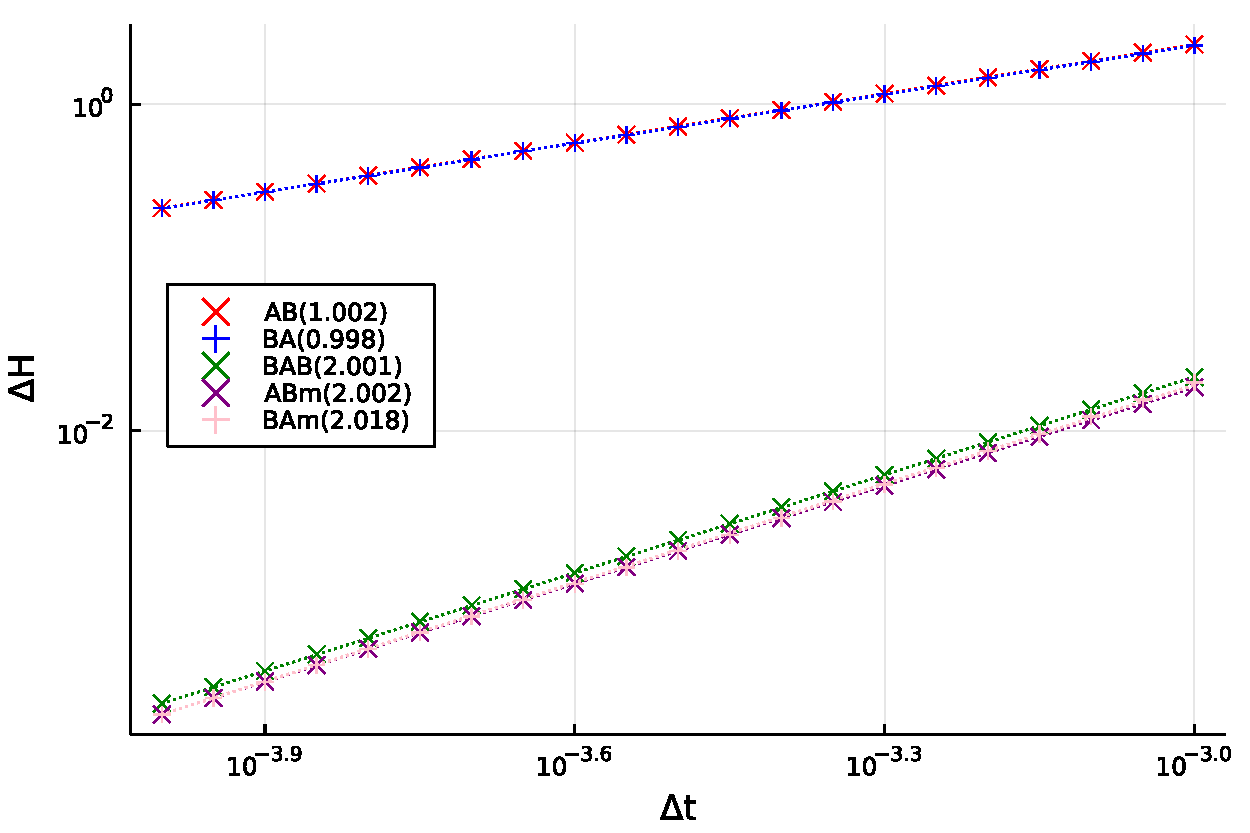
\includegraphics[width=0.85\linewidth]{figures/chapter1/energy_conservation.pdf}
          \caption{ \label{fig:hamiltonian_conservation}
            Maximal fluctuation of the Hamiltonians and leading-order modified Hamiltonians for the Symplectic Euler and Verlet schemes.
          }
        \end{center}
      \end{figure}

    From a practical point of view, we will always use the Verlet scheme, 
    since it offers the better energy conservation property without any computational overhead compared to the symplectic Euler schemes. 
    Indeed, the force calculation in the last step of \eqref{eq:verlet} can be used again in the first step of the next iteration, so that there is only one force calculation per iteration, as in the symplectic Euler method.
    Finally let us mention that the splitting based on the ordering $ABA$ of the elementary generators yields another symplectic method called the \textit{position} Verlet scheme, which enjoys the same conservation properties as standard (velocity) Verlet.
    It is, however, rarely used in practice.

\section{Canonical averages}
We now turn our attention to methods to compute canonical averages, which are expectations of observables with respect to the canonical measure \eqref{eq:canonical_measure}.
As we already alluded to, the sampling strategy will be based on the definition of a stochastic process under whose evolution the canonical measure is invariant. This is the Langevin dynamics.
We define it, and discuss some of its theoretical properties which are relevant to the sampling of canonical averages.
We then turn to describing a splitting strategy for the discretization of the continuous dynamics, which will serve as our effective sampling tools for canonical averages.
We finally give some numerical illustrations of the strategy.
\subsection{Langevin dynamics}
We first consider the inertial Langevin dynamics, defined by the following stochastic differential equation (SDE), where $\gamma, \beta$ are fixed positive constants:
\begin{equation}
    \label{eq:langevin}
    \left\{\begin{aligned}
        \text dq_t&=M^{-1}p_t\,\dt,\\
        \text dp_t&= -\nabla V(q_t)\,\dt -\gamma M^{-1}p_t\,\dt+\sqrt{\frac{2\gamma}\beta}\text \,dW_t,
    \end{aligned}\right.
\end{equation}
where $(W_t)_{t\geq 0}$ is a standard $dN$-dimensional Brownian motion.
This process is a combination of a Hamiltonian evolution with an additional action on the momenta which, if isolated, defines a $dN$-dimensional Ornstein-Uhlenbeck process.

This additional term be interpreted physically as the combination of two effects: a dissipation term 
$$-\gamma M^{-1}p_t\dt,$$
which can be understood as the effect of a viscous friction force on the particles, and a fluctuation term, 
$$\sqrt{\frac{2\gamma}\beta}\text dW_t,$$
which corresponds to the input of kinetic energy into the system as thermal agitation induced by a surrounding heat bath at temperature $1/(k_B\beta)$.\\

However, the physical meaning can be forgotten thanks to the fact that, \textit{in fine}, we only require that the canonical measure be invariant under this dynamic: as we shall shortly see, this is indeed the case.

\begin{remark}[Generalized Langevin dynamics]
    There are several ways to generalize this process: one is to consider a generic, possibly non-separable, Hamiltonians, as in Remark \ref{rem:non_separable_hamiltonian}, rather than the classical Hamiltonian used above.
    The other is to allow the fluctuation-dissipation term to be parametrized by coefficients $\gamma$ and $\sigma$ depending on the state variable, and which obey a relation ensuring the invariance of $\mu$.
    Hence in full generality, we could consider the following system of SDEs:
    \begin{equation}
        \label{eq:general_langevin}
        \left\{\begin{aligned}
            \text dq_t &=\nabla_p H(q_t,p_t)\dt,\\
            \text dp_t &= -\nabla_q H(q_t,p_t)\dt -\gamma(q_t,p_t)\nabla_pH(q_t,p_t)\dt+\sigma(q_t,p_t)\rm{d}W_t,
        \end{aligned}\right.
    \end{equation}
    where $\gamma$ and $\sigma$ are $dN \times dN$ matrix-valued functions.
    In fact one can also consider the case where $W_t$ is a $r$-dimensional Brownian motion and $\sigma$ is a $dN\times r$ matrix-valued function.
    The Dissipative Particle Dynamics (DPD, see \cite{EW95}) is a generalized Langevin equation of this form, where $\gamma$ and $\sigma$ are position-dependent and the Brownian motion is $dN(N-1)/2$-dimensional, which corresponds to the number of pairs of non-orthogonal momentum degrees of freedom.
\end{remark}

The generator of the Langevin dynamics is the operator
\begin{equation}
  \label{eq:langevin_generator}
\mathcal L_\gamma=M^{-1}p\cdot \nabla_q-\nabla V(q) \cdot \nabla_p- \gamma M^{-1} p \cdot \nabla_p+\frac\gamma\beta \Delta_p,
\end{equation}
and we denote the evolution operator using exponential notation:
\begin{equation}
    \label{eq:langevin_evolution_operator}
    \left(\e^{t\cL_\gamma}\varphi\right)(q,p) \defeq \E^{(q,p)}\left[\varphi(q_t,p_t)\right],
\end{equation}
where the expectation is over all trajectories of the dynamics \eqref{eq:langevin}, starting from $(q_0,p_0)=(q,p)$.

    \subsection{Invariance of the canonical measure}

    Using the generator, one can easily express the evolution of a probability distribution under the Langevin dynamics.
    We assume for simplicity that the solution $(q_t,p_t)_{t\geq 0}$ to \eqref{eq:langevin} has a distribution with a smooth density $\rho_t$ at time $t$ over $\mathcal E$.
    For any $C^\infty$ compactly supported observable $\varphi$, we have
    $$\int_{\mathcal E}\varphi(q,p)\rho_t(q,p)\,\dif q\,\dif p=\int_{\mathcal E}\E^{(q,p)}\left[\varphi(q_t,p_t)\right]\rho_0(q,p)\dif q\dif p=\int_{\mathcal E}\mathrm{e}^{t\cL_\gamma}\varphi(q,p)\rho_0(q,p)\dif q\dif p,$$
    where the superscript is as in \eqref{eq:invariant_measure}. Thus,
    $$\frac{\partial}{\partial t}\left(\int_{\mathcal E}\varphi(q,p)\rho_t(q,p)\,\dif q\,\dif p\right)=\int_{\mathcal E}\mathrm{e}^{t\cL_\gamma}\cL\varphi(q,p)\rho_0(q,p)\,\dif q\,\dif p=\int_{\mathcal E}\cL_\gamma\varphi(q,p)\rho_t(q,p)\,\dif q\,\dif p$$
    If we define $\cL_\gamma^\dagger$ as the adjoint of $\cL_\gamma$ on the flat space $L^2(\mathcal E)$, that is,
    \begin{equation}
        \label{eq:L_dagger}
        \int_{\mathcal E}\left(\cL_\gamma\varphi\right)\psi=\int_{\mathcal E}\varphi \left(\cL_\gamma^\dagger \psi\right)\qquad\text{for all }\phi,\,\psi
    \end{equation}
     compactly supported $C^\infty$ test functions, we have the Fokker--Planck equation,
    \begin{equation}\label{eq:fokker_planck}
        \frac{\partial}{\partial t}\int_{\mathcal E}\varphi(q,p)\rho_t(q,p)\dif q\dif p=\int_{\mathcal E}\varphi(q,p)\cL_\gamma^\dagger\rho_t(q,p)\dif q \dif p,
    \end{equation}
    which rewrites formally as 
    \begin{equation}
        \label{eq:fokker_planck_formal}
        \frac{\partial}{\partial t}\rho_t=\cL_\gamma^\dagger\rho_t.
    \end{equation}
    Using this equation, we can easily show that the canonical distribution is invariant under this dynamics, which is equivalent to the condition 
    $$\cL_\gamma^\dagger \mu=0.$$
    In fact, it is useful to reformulate this condition in the weighted space $L^{2}(\mu)$. Indeed, the stationary Fokker--Planck equation rewrites
    $$\int_{\mathcal E}\cL_\gamma \varphi \,\dif \mu=0\qquad \forall\,\varphi,$$
    or equivalently,
    $$\cL_\gamma^* \1_{\mathcal E}=0,$$
    where $\cL_\gamma^*$ is the adjoint of $\cL_\gamma$ in $L^2(\mu)$ for the scalar product
    $$(\varphi,\psi)\mapsto \int_{\mathcal E}\varphi \psi \,\dif \mu.$$
    This, in turn, follows easily from the following lemma.
    \begin{lemma}
        \label{lemma:star_adjoints_langevin}
        The $L^2(\mu)$ adjoints of the elementary differential operators are given by the formulae
        \begin{equation}
            \label{eq:star_adjoints_langevin}
            \left\{\begin{aligned}
            &\partial_{q_i}^*=-\partial_{q_i}+\beta\partial_{q_i}V,\\
            &\partial_{p_i}^*=-\partial_{p_i}+\beta\left(M^{-1}p\right)_i.
            \end{aligned}\right.
        \end{equation}
    \end{lemma}
    These are easily found by integration by parts. In particular, we find that 
    $$\partial_{q_i}\partial_{p_i}^*-\partial_{p_i}\partial_{q_i}^*=\beta\left((M^{-1}p)_i\partial_{q_i}-\partial_{q_i}V\partial_{p_i}\right),$$
    hence, by summing over $i$,
    \begin{equation}
        \label{eq:L_ham_antisymmetric}
        \cLham=\frac1\beta\left(\nabla_q\cdot\nabla_p^*-\nabla_p\cdot\nabla_q^*\right),
    \end{equation}
    which is an antisymmetric operator. Similarly,
    $$\partial_{p_i}\partial_{p_i}^*=\beta(M^{-1}p)_i\partial_{p_i}-\partial_{p_i}^2,$$
    hence
    \begin{equation}
        \label{eq:C_symmetric}
        C=-\frac{1}\beta\nabla_p\cdot\nabla_p^*,
    \end{equation}
    which is a symmetric operator. In summary, we have that 
    \begin{equation}
        \label{eq:L_star}
        \cL_\gamma^*=-\cLham+\gamma C=-(A+B)+\gamma C.
    \end{equation}
    It follows immediately that $\cL_\gamma^*\1_{\mathcal E}=0$. Notice that since $\cLham^*\1_{\mathcal E}=0$, the canonical measure is also invariant under the Hamiltonian dynamics. However, because the latter is restricted to a manifold with zero measure with respect to $\mu$, Hamiltonian ergodic averages cannot in general converge to the correct value.
    \begin{remark}[Fluctuation-dissipation relation for generalized Langevin dynamics]
        We come back to the general Langevin dynamics \eqref{eq:general_langevin}.
        In this case the generator is given by 
        \[\cL_{\gamma,\sigma}=\cLham-(\gamma \nabla_p H)\cdot \nabla_p +\frac12(\sigma \sigma^\intercal) : \nabla_p^2.\]
        The canonical measure is invariant under the action of the Hamiltonian part, so having
        \[\widetilde{\cL}_{\mathrm{FD}}\defeq -(\gamma \nabla_p H)\cdot \nabla_p +\frac12(\sigma \sigma^\intercal) : \nabla_p^2 \]
        such that  $\widetilde{\cL}_{\mathrm{FD}}^*\1_\mathcal{E}=0$ is enough to guarantee the invariance of the canonical measure.
        If $\gamma$ and $\sigma$ are momentum-dependent, then this condition is a complicated differential-in-$p$ relation between the coefficients of $\gamma$ and $\sigma$, which can be explicitly computed by integration by parts in the expression
        \[\int_{\mathcal E} (\cL_{\mathrm{FD}}\varphi)\psi\e^{-\beta H},\]
        with $\varphi, \psi \in C_c^\infty(\mathcal E)$ test functions. 
        In the case where $\gamma$ and $\sigma$ are only position-dependent however, as is often the case in practice, then the expression simplifies greatly, and becomes simply an algebraic relationship between $\gamma$ and $\sigma$, namely
        \begin{equation}
            \label{eq:general_fd_relation}
            \sigma \sigma^\intercal =\frac{2\gamma}{\beta}.
        \end{equation}
    \end{remark}

    \subsection{Overdamped limit of Langevin dynamics}
        As already pointed out, the fact that the kinetic marginal of $\mu$ is a Gaussian distribution makes sampling canonical momenta trivial. 
        Instead, the main problem is sampling from $\nu$. It follows directly from the invariance of $\mu$ under trajectories of the Langevin dynamics that $\nu$ is invariant under the configurational trajectories of the Langevin dynamics.
        It would be convenient, however, to have at our disposal a dynamics on $\mathcal D$ which has $\nu$ as an invariant measure.
        It turns out this is possible, by observing that the invariance of $\mu$ is independent of the parameter $\gamma$, and taking the limit $\gamma\to\infty$. This requires a bit of care.
        Notice the SDE on the momenta in \eqref{eq:langevin} rewrites 
        \[\dif p_t=-\nabla V(q_t)\dif t-\gamma \dif q_t+\sqrt{\frac{2\gamma}\beta}\dif W_t,\]
        thus a time integration gives
        \[q_t-q_0=\frac{p_0-p_t}\gamma -\frac{1}\gamma\int_0^t\nabla V(q_s)\dif s +\sqrt{\frac{2}{\gamma\beta}}W_t.\]
        The scaling invariance of the Brownian motion $(\sqrt{\alpha}W_{t/\alpha^2})_{t\geq 0}\sim (W_t)_{t\geq 0}$ suggests considering the timescale $\gamma\beta t$, thus
        \[q_{\gamma\beta t}-q_0=\frac{p_0-p_{\gamma\beta t}}\gamma-\frac1{\gamma}\int_0^{\gamma\beta t}\nabla V(q_s)\dif s +\sqrt{2}\widetilde{W_t},\]
        where $\widetilde W$ is again a Brownian motion. Using the change of variables $s=\gamma \beta u$ in the integral term yields
        \begin{equation}\label{eq:rescaled_langevin}q_{\gamma\beta t}-q_0=\frac{p_0-p_{\gamma\beta t}}\gamma-\beta\int_0^{t}\nabla V(q_{\gamma\beta u})\dif u +\sqrt{2}\widetilde{W_t},\end{equation}
        At this point, we formally take $\gamma\to\infty$, which suggests the following SDE for the rescaled in time process,
        \begin{equation}
            \label{eq:overdamped_langevin}
            \dif q_t=-\beta \nabla V(q_t)\,\dif t+\sqrt{2}\,\dif W_t.
        \end{equation}
        
        This equation defines the overdamped Langevin, or Brownian, dynamics.
        To justify the limit in a rigorous manner, one would hope to show that the rescaled process \eqref{eq:rescaled_langevin} converges in law to a weak solution of the SDE \eqref{eq:overdamped_langevin}, in some functional space.
        However, this is technical overkill, since, we only need to consider dynamics as sampling devices. In fact, the physical interpretation of this equation is not entirely clear in terms of the dimensions of the quantities involved.
        We can just as well take equation \eqref{eq:overdamped_langevin} as given, and be satisfied by the following fact.
    
        \begin{prop}
            The configurational Gibbs measure $\nu$ is invariant under the dynamics \eqref{eq:overdamped_langevin}.
        \end{prop}
    
        This follows along the same lines as for the Langevin dynamics. The generator (now acting on observables defined on $\mathcal D$) is the operator
        \begin{equation}
            \label{eq:overdamped_langevin_generator}
            \cL\varphi=-\beta\nabla V\cdot \nabla\varphi + \Delta \varphi.
        \end{equation}
        Again, we consider the weighted space $L^2(\nu)$. Adjoints of elementary differential operators are still given by the first line of \eqref{eq:star_adjoints_langevin}, and it is then easily seen that
        \begin{equation}
            \label{eq:L_overdamped_symmetric}
            \cL=-\nabla^*\cdot\nabla
        \end{equation}
        is a symmetric operator. Again we have $\cL^*\1_{\mathcal D}=0$, so $\nu$ satisfies the stationary Fokker--Planck equation under this dynamics.
    
        \begin{remark}
            Instead of rescaling time by $\beta\gamma$, we could have rescaled by $\gamma$, which would yield the dynamics
            \begin{equation}
                \label{eq:overdamped_langevin_alt}
                \dif q_t=-\nabla V(q_t)\dif t+\sqrt{\frac 2\beta}\dif W_t.
            \end{equation}
            Which formulation to choose is a matter of preference, since both yield a dynamics invariant under $\nu$, as seen from the identity (where we still write $\cL$ for the generator)
            \[\cL=-\frac1\beta\nabla^*\cdot\nabla.\]
        \end{remark}
        We end this chapter by stating some key properties of the continuous dynamics, regarding ergodicity and and statistical error, before moving to the description of splitting schemes. 

        \subsection{Convergence to equilibrium}
        Once we have shown that the Langevin dynamics and its overdamped limit are reasonable candidates to sample from the canonical measure and its configurational marginal,
        we should ensure that the target measure is actually sampled, and not simply invariant for the dynamics, as the cautionary example of the Hamiltonian dynamics shows.
        This is the question of ergodicity, and resuts of this nature mainly come in two flavors.
        \begin{enumerate}[(i)]
            \item Probabilistic ergodic theorems that ask about the convergence of random variables like \eqref{eq:ergodic_averages}, that give analogs of the Law of Large Numbers for the correlated process $\varphi(q_t,p_t)$.
            \item More analytic results which express the convergence of the law of the process at time $t$ towards a stationary solution to the Fokker--Planck equation. These can usually be expressed as decay estimates on the evolution Semigroup \eqref{eq:langevin_evolution_operator}, in a judiciously chosen functional setting.
        \end{enumerate}
        We will not get into details as these questions can quickly get quite technical, but rather give intuitive ideas of the setting, and point the reader to more thorough sources.
        Results such as (i) typically leverage the strong Law of Large Numbers by dissecting the trajectory into a discrete number of (loosely) \iid excursions through phase space, guaranteeing the almost sure convergence of trajectory averages.
        As such, proving the positive recurrence of the dynamics is crucial to showing that these excursions are well-behaved, while also implying that the invariant measure is unique.
        One idea, exploited by Kliemann in \cite{K87}, is to recast the Langevin dynamics as a control equation (where $W_t$ acts as the control). 
        He is thus able to leverage criteria on $\cL_\gamma$ from geometric control theory to ensure the almost sure convergence of trajectory averages.
        Results such as (ii) depend on the functional setting. Let us simply state the following result, based on hypocoercive estimates. 
        For an introduction to these ideas, and references, we point to Section 2.1.1 in \cite{LMS13}, and \cite[DMS15].
        For any measure $\rho$ denote by $L^2_0(\rho)$ the space of centered $L^2$ observables with respect to $\rho$.
        \begin{prop}[Exponential decay rate of the Semigroup]
            Assume that the potential $V$ is smooth and that the configurational marginal $\nu$ of $\mu$ satisfies a Poincaré inequality:
            there exists a constant $R>0$ such that for all $\varphi \in L^2_0(\nu)$ such that $\nabla \varphi \in L^2(\nu)^{dN}$,
            \begin{equation}
                \label{eq:poincare_inequality}
                \|\varphi \|_{L^2(\nu)}^2\leq \frac1R \| \nabla \varphi\|^2_{L^2(\nu)}.
            \end{equation}
            Then there exist constants $C_\gamma,\lambda_\gamma >0$ such that 
            \begin{equation}
                \label{eq:semigroup_exp_decay}
                \|\e^{t\cL_\gamma}\|_{\mathcal{B}(L^2(\mu))}\leq C_\gamma \e^{-t\lambda_\gamma}.
            \end{equation}
        \end{prop}
        For the overdamped case, exponential decay rates can also be obtained (much more directly) under the same conditions.
        Moreover the Poincaré inequality \eqref{eq:poincare_inequality} is automatically satisfied in the case of a compact configurational space $\mathcal D$.
        
        \subsection{Asymptotic variance for ergodic averages}\label{subsec:asymptotic_variance_cont}
        Since ergodic averages are computed over a finite time-interval, the corresponding random variable will have some variance. 
        Let us show how to relate this variance to the dynamics, provided a Central Limit Theorem holds.
        For simplicity, we assume that $(q_0,p_0)\sim \mu$, and let $\varphi \in H^1(\mu)$ be an observable of interest. We also denote by
        \begin{equation}
            \label{eq:equilibrium_projector}
            \Pi \varphi = \varphi -\int_\mathcal{E}\varphi\,\dif \mu
        \end{equation}
        the centering projector associated with $\mu$. The Central Limit Theorem asserts that the following convergence in law holds:
        \begin{equation}
            \label{eq:clt_diffusion}
            \frac1{\sqrt{T}}\int_0^T\Pi\varphi(q_t,p_t)\,\dif t \overset{\mathrm{law}}{\implies} \mathcal N(0,\sigma_{\varphi}^2),
        \end{equation}
        where $\sigma_{\varphi}^2$ is the asymptotic variance associated to $\varphi$ under the dynamics, which is thus given by the limit of the variance on the left-hand side. Let us compute:
        \[\sigma_{\varphi,T}^2\defeq \E_\mu\left[\left(\frac1{\sqrt{T}}\int_0^T\Pi\varphi(q_t,p_t)\,\dif t\right)^2\right]=\frac1T\int_0^T\int_0^T\E_\mu\left[\Pi\varphi(q_t,p_t)\Pi\varphi(q_s,p_s)\right]\,\dif s\,\dif t.\]
        By stationarity, for $t>s$, $\Pi\varphi(q_t,p_t)\Pi\varphi(q_s,p_s)\sim \Pi\varphi(q_{t-s},p_{t-s})\Pi\varphi(q_0,p_0)$, hence we may write, by Fubini's theorem, 
        \begin{align*}\sigma_T &= \frac2T\int_0^T\int_0^t\E_\mu\left[\Pi\varphi(q_{t-s},p_{t-s})\Pi\varphi(q_0,p_0)\right]\,\dif s\,\dif t\\
             &= \frac2T\int_0^T\int_s^T\E_\mu\left[\Pi\varphi(q_{s},p_{s})\Pi\varphi(q_0,p_0)\right]\,\dif t\,\dif s\\
             &=2\int_0^T\E_\mu\left[\Pi\varphi(q_{s},p_{s})\Pi\varphi(q_0,p_0)\right]\left(1-\frac{s}{T}\right)\,\dif s\\
             &=2\int_0^T\E_\mu\left[\left(e^{s\cL_\gamma}\Pi\varphi\right)\left(\Pi\varphi\right)\right]\left(1-\frac{s}{T}\right)\,\dif s
        \end{align*}
        Using a Cauchy--Schwarz inequality in $L^2(\mu)$ and an exponential decay estimate on the evolution semigroup like \eqref{eq:semigroup_exp_decay}, we obtain a bound of the form
        \[\int_0^T\left|\E_\mu\left[\left(e^{s\cL_\gamma}\Pi\varphi\right)\left(\Pi\varphi\right)\right]\frac{s}{T}\right|\,\dif s\leq \int_0^\infty C_\gamma\e^{-\lambda_\gamma s}\left\|\Pi\varphi\right\|^2_{L^2(\mu)}\frac{s}{T}\,\dif s\]
        for some positive constants $C$ and $\alpha$, which converges uniformly to $0$ as $T\to \infty$. It follows that 
        \begin{equation}
            \label{eq:asymptotic_variance_with_semigroup}
            \sigma_{\varphi}^2=\int_0^\infty \E_\mu\left[\left(e^{s\cL_\gamma}\Pi\varphi\right)\left(\Pi\varphi\right)\right]\,\dif s.
        \end{equation}
        We use the following equality of bounded operators on $\mathcal{H}^1(\mu)$, which is the operator:
        \begin{equation}
            \label{eq:resolvent_langevin}
            (-\cL_\gamma)^{-1}=\int_0^\infty \e^{s\cL_\gamma}\,\dif s,
        \end{equation}
        which again is justified by the exponential decay rate of evolution semigroup, and where the integral on the right is in the Bochner sense, that is a generalization of the Lebesgue integral to functions taking values in a general Banach space.
        Using this identity, we can write the asymptotic variance more concisely,
        \begin{equation}
            \label{eq:asymptotic_variance_with_Lm1}
            \sigma_{\varphi}^2=\E_{\mu}\left[(\Pi\varphi) (-\cL_\gamma)^{-1}(\Pi \varphi)\right].
        \end{equation}
        Note that the exact same computations can be performed for the overdamped Langevin dynamics. 
        It follows from \cite[Theorem 2.1]{B82}, that a sufficient condition for a CLT to hold is that $\Pi \varphi\in \operatorname{Ran}\mathcal L_\gamma$, which is the case provided we can express the inverse of $\cL_\gamma$ using \eqref{eq:resolvent_langevin}.
\subsection{Splitting schemes for the Langevin dynamics}\label{section:splitting_schemes_langevin}

Similarly to the Hamiltonian case, the generator \eqref{eq:langevin_generator} splits into three elementary generators, namely 
$$\mathcal L_\gamma= A+B+\gamma C=\cLham +\gamma C,$$
with
\begin{equation}
  \label{eq:C_definition}
C=-M^{-1}p\cdot \nabla_p +\frac1\beta \Delta_p.
\end{equation}
These generators individually give rise to dynamics which we can analytically integrate, defined by the following evolution operators:

\begin{equation}
  \label{eq:propagators}
  \left\{\begin{aligned}
    &\mathrm{e}^{tA}\varphi(q,p)=\varphi(q+tM^{-1}p,p),\\
    &\mathrm{e}^{tB}\varphi(q,p)=\varphi(q,p-t\nabla V(q)),\\
   &\mathrm{e}^{t\gamma C}\varphi(q,p)=\mathbbm E \left[\varphi \left(q, \mathrm e^{-\gamma M^{-1}t}p + \sqrt{\frac{M}{\beta}(1-\mathrm{e}^{-2\gamma M^{-1}t})}G\right)\right],
\end{aligned}\right.
\end{equation}
where $G$ is a standard $dN$-dimensional Gaussian. The third equality is a reformulation of an equality in law between an Itô integral and a Gaussian random variable, and follows by applying Itô's formula to the rescaled process
$$\e^{\gamma M^{-1}t}p_t,$$
where $p_t$ is the Ornstein--Uhlenbeck process:
\begin{equation}
    \dif p_t=-\gamma M^{-1}p_t\,\dif t+\sqrt{\frac{2\gamma}{\beta}}\,\dif W_t,
\end{equation}
then applying the following matrix form of Itô's isometric property 
\begin{equation}
    \label{eq:ito_isometry_matrix}
    \int_0^t A_s\,\dif W_s \overset{\mathrm{law}}{=} \left(\int_0^t A_s A_s^\intercal \,\dif s\right)^{\frac12}\mathcal G
\end{equation}
to obtain the equality in law.
 The dynamics associated with the $A$ and $B$ parts are deterministic Hamiltonian dynamics already identified in \eqref{eq:Lham_splitting_dynamics_solved}.
Just as in the Hamiltonian case, we can define schemes for the Langevin dynamics based on approximating the evolution operator \eqref{eq:langevin_evolution_operator} over one timestep by splitting the generator $\cL_\gamma$, and combining the corresponding evolution operators \eqref{eq:propagators} in a sequence.
We refer to such a splitting approximation by the sequence in which the individual propagators are composed. It is useful at this point to introduce the stochastic flow map associated with the Ornstein--Uhlenbeck dynamics.
\begin{equation}
    \label{eq:stochastic_flow_c}
    \Phi_t^C(q,p,\xi)=\left(q, \mathrm e^{-\gamma M^{-1}t}p + \sqrt{\frac{M}{\beta}(1-\mathrm{e}^{-2\gamma M^{-1}t})}\xi\right),
\end{equation}
where $\xi\in \R^{dN}$. The map is defined so that $\E[\varphi\left(\Phi_t^C(q,p,G)\right)]=\mathrm{e}^{t\gamma C}\varphi(q,p)$ when $G$ is a standard Gaussian random variable.
Given an ordering of operators, 
\begin{equation}\label{eq:splitting_ordering}(R_1,\dots,R_k)\in \{A,B,\gamma C\}^k,\end{equation}
we can consider the mapping obtained by composing the elementary flows, noted as
\begin{equation}\label{eq:markov_mapping}\Phi^{R_1,\dots R_k}\defeq\Phi_{\Delta t/n_{R_k}}^{R_k}\circ\dots\circ\Phi_{\Delta t/n_{R_1}}^{R_1},
\end{equation}
where
$$n_R\defeq \#\left\{1\leq j\leq n \middle| R_j=R\right\}$$
for $R\in\{A,B,\gamma C\}$, and which we may consider by a slight abuse to be the mapping which takes a point in phase space and $n_{\gamma C}$ vectors in $\xi_1,\dots,\xi_{n_{\gamma C}}\in\R^{dN}$, yielding a point in phase space by successively applying the flow, and, if need be, stochastic flow, mappings corresponding to the reverse ordering of \eqref{eq:splitting_ordering}.
Applying this mapping with a vector of independent standard Gaussians yields a stochastic mapping, which defines the update rule for the splitting scheme associated with the ordering \eqref{eq:splitting_ordering}.
An important property which follows from writing the update rule using the mapping \eqref{eq:markov_mapping} is that numerical trajectories formed by iterating this update rule with independent vectors of standard Gaussians form a Markov chain.
The hope is that the invariant measure corresponding to this Markov chain (provided it is unique) is a close approximation to the canonical measure, as well as being ergodic.
It is less cumbersome to write such schemes at the level of the evolution operator associated with the Markov chain,

\begin{equation}
    \label{eq:markov_evolution_operator}
    P_\Dt\varphi (q,p) = \E\left[\varphi(q^1,p^1)\middle|q^0=q,\,p^0=p\right].
\end{equation}
The evolution operator associated with the splitting \eqref{eq:splitting_ordering} is
\begin{equation}
    \label{eq:splitting_semigroup_expr}
    P_\Dt=\e^{\Dt/n_{R_1}R_1}\dotsm\e^{\Dt/n_{R_k}R_k}.
\end{equation}
Note that the order is reversed compared to the stochastic flow formulation.
While the formulation at the stochastic flow level is slightly complicated to write, it corresponds very closely to how a general splitting integrator for the Langevin dynamics can be implemented.
One simply has to compute the timestep corresponding to each operator in the ordering, and apply in succesive steps the corresponding flow maps, sampling independent Gaussian variables for each stochastic step.
We will refer to such schemes by the name obtained by concatenating the names of each operator appearing in the ordering, using $O$ instead of $\gamma C$.
For instance, the BAOAB scheme corresponds to the case $k=5$, $n_A=n_B=2$, and $n_{\gamma C}=1$, and the ordering $(B,A,\gamma C,A,B)$.
    \begin{example}[BAOAB scheme]
        The update rule is given by the following equations, with additional intermediate coordinate and momentum variables:
        \begin{equation}\label{baoab}
            \left\{\begin{aligned}
                 p^{n+\frac13} &=p^n -\frac{\Delta t}{2}\nabla V(q^n)\\
                 q^{n+\frac12} &=q^n + \frac{\Delta t}{2} M^{-1}p^{n+\frac 13}\\
                 p^{n+\frac23} &=\alpha_{\Delta t}p^{n+\frac13}+\sigma_{\Delta t}G^n\\
                 q^{n+1} &=q^{n+\frac12} + \frac{\Delta t}{2} M^{-1}p^{n+\frac 23}\\
                 p^{n+1} &= p^{n+\frac23}-\frac{\Delta t}{2}\nabla V(q^{n+1}),
            \end{aligned}\right.
        \end{equation}
        where, again, $G^n$ is a standard $dN$-dimensional Gaussian.
    \end{example}
     Now we have a recipe to make an infinite number of numerical schemes, which can easily be implemented in a computer.
     We could even go further and consider methods with an uneven distribution for the secondary timesteps, the introduction of negative secondary timesteps for the $A$ and $B$ steps, and so on.
     This room for creativity highlights the need for criteria to assess the quality of such schemes. A tradeoff between various considerations has to be found:

     \begin{enumerate}[(i)]
         \item Our aim is to compute long trajectories, which are needed to ensure that the phase space is properly explored, as well as to obtain better statistical properties for averages \eqref{eq:discrete_ergodic_averages}. Thus, for a fixed computational budget, we desire a scheme which allows us to take as large a timestep $\Delta t$ as possible. This is the issue of numerical stability.
         \item The use of a positive timestep $\Delta t$ implies in general that the invariant measure for the Markov chain corresponding to a given scheme is not the canonical measure. This issue is called systematic error, or bias, and one would desire a scheme which minimizes this bias.
         \item The main computational cost in computing iterates of these numerical schemes is the evaluation of the gradient of the potential used for the $B$ steps. As such, it is desirable to have a scheme which requires as few evaluations of this gradient as possible per iteration. Some care must be taken when implementing these, to ensure that already computed gradients are not re-computed: for instance, the gradient in the last step of the BOAB scheme, is equal to the one in the first step of the next iteration.
         \item Notice that the parameter $\gamma$ is free for the practitioner to choose. A natural question is to determine the properties of the marginal dynamics in $q$ in the limit $\gamma \to +\infty$, and in particular if we obtain a consistent discretization of the overdamped Langevin dynamics. Conversely, one could ask about properties of the dynamics as we take the Hamiltonian limit $\gamma\to 0$.
     \end{enumerate}

     \begin{remark}[Overdamped and Hamiltonian limits in splitting schemes]
        Concern (iv) is simple to address. Since
        \[\underset{\gamma \to 0}{\lim}\,\alpha_\Dt=1\,\qquad \underset{\gamma \to +\infty}{\lim}\alpha_\Dt=0,\]
        every $O$-step can simply be dropped as $\gamma\to 0$ from the sequence of operators defining the splitting. 
        This yields a symplectic scheme for the Hamiltonian parts of the dynamics, whose properties can be analyzed as before.
        For this reason, the ordering of the Hamiltonian parts of the splitting of most commonly used schemes corresponds to that of a velocity Verlet method.
         As $\gamma \to \infty$, 
        every $O$-step reduces to resampling the momentum according to the Maxwell--Boltzmann distribution. 
        The properties of the resulting scheme depend on the particular ordering of the splitting at hand. 
        For instance, if every $A$ step is preceded by an $O$ step, then the potential is entirely ignored by the evolution, and the trajectories form an isotropic random walk. This is for instance the case of the BOA scheme.
        On the other hand, it may happen that one obtains a discretization of the overdamped Langevin dynamics. For example, the update equation for the overdamped limit of the BAOA scheme in the case $M=\Id$ rewrites
        \[q^{n+1}=q^n -\frac{\Dt^2}2\nabla V(q^n)+\frac12\sqrt{\frac{\Dt^2}\beta}\left(G^n+G^{n+1}\right),\]
        with $(G^n)$ an \iid standard Gaussian sequence. Because of the two-step correlations in the Gaussian increments, the numerical trajectories are not Markovian as such.
        Nevertheless the scheme is reminiscent of a discretization of the overdamped equation \eqref{eq:overdamped_langevin_alt}, but with an effective timestep $\frac{\Dt^2}2$. 
        This quadratic rescaling of the timestep is common, and has to be related to the fact that the overdamped equation is defined through a diffusive rescaling.
        This discretization also corresponds to the overdamped limit of the BAOAB scheme, which is unsurprising in view of the results of the next chapter.
     \end{remark}

    \subsection{Error analysis for splitting schemes}
        We turn our attention to analyzing the error arising from the estimation of canonical expectations by discrete ergodic averages. We consider estimations of the form 
        \[\widehat{\varphi}_{N_{\mathrm{iter}}} \defeq \frac1{N_{\mathrm{iter}}}\sum_{k=0}^{N_{\mathrm{iter}}-1}\varphi(q^k,p^k),\]
        where $(q^n,p^n)_{n\geq 0}$ is a numerical trajectory of a Markov chain which is ergodic with respect to a unique stationary distribution $\mu_{\Dt}$ on $\mathcal E$, which approximates $\mu$.
        To show the existence of such an invariant distribution, one can rely on general results from the theory of Markov chains, combined with Lyapunov estimates. For a precise result, we refer the reader to \cite[Proposition 2.9]{LMS13}, for example.
        For simplicity, we will assume that $(q^0,p^0)$ is distributed according to $\pi_\Dt$, so that the whole numerical trajectory is stationary. This requires in practice that the system be equilibriated before starting to sample the observables of interest. We decompose the error as follows:
        \begin{equation}\label{eq:error_decomposition}\widehat{\varphi}_{N_{\mathrm{iter}}}-\int_\mathcal{E}\varphi \,\dif \mu= \widehat{\varphi}_{N_{\mathrm{iter}}} - \int_\mathcal{E}\varphi \,\dif \mu_{\Dt}+\int_\mathcal{E}\varphi\,\dif \mu_{\Dt}-\int_{\mathcal E}\varphi \,\dif \mu.\end{equation}
        Two terms contribute to the error.
        \subsubsection{Statistical Error}
        The first term
        \[\widehat{\varphi}_{N_{\mathrm{iter}}} - \int_\mathcal{E}\varphi \,\dif \mu_{\Dt}\]
        is the statistical error due to the truncation of computed trajectories to a finite time $T_{\mathrm{sim}}\defeq N_{\mathrm{iter}}\Dt$. 
        By the Central Limit Theorem for Markov Chains, asymptotically, the statistical error is of order
        $\sigma_{\varphi,\Dt}/\sqrt{N_{\mathrm{iter}}}$,
        where $\sigma_{\varphi,\Dt}$ is the asymptotic variance of the Markov chain, which is given by the following expression, under suitable assumptions, by
        \[\sigma_{\varphi,\Dt}^2=\mathrm{Var}_{\pi_\Dt}(\varphi)+2\sum_{k=1}^\infty \mathrm{Cov}_{\pi_\Dt}(\varphi(q^0,p^0)\varphi(q^k,p^k)).\]
        The proof of the above expression is in spirit the same as the one in the continuous case, exploiting the stationarity in law of the trajectory.
        Using the evolution and projection operators associated with the Markov chain, which are respectively defined by
        \begin{equation}
            \label{eq:markov_chain_operators}
            P_{\Dt}\varphi(q,p)=\E[\varphi(q^1,p^1)|(q^0,p^0)=(q,p)],\qquad \Pi_\Dt \varphi=\varphi - \int_{\mathcal E}\varphi \,\dif \mu_{\Dt},
        \end{equation}
        we can rewrite the asymptotic variance in a more analytic form, namely
        \begin{equation}
            \label{eq:asymptotic_variance_markov_chain}
            \sigma_{\varphi,\Dt}^2=2\int_{\mathcal E}(\Pi_{\Dt}\varphi)(\Id-P_\Dt)^{-1}(\Pi_\Dt \varphi)\,\dif\mu_{\Dt}-\int_{\mathcal E}(\Pi_\Dt \varphi)^2\,\dif \pi_\Dt,
        \end{equation}
        where we formally used the Neumann series
        \[\sum_{k=0}^\infty P_\Dt=(\Id-P_\Dt)^{-1},\]
        which has to justified rigorously, for instance using the geometric decay estimate for $P_\Dt^n$ from \cite[Proposition 2.9]{LMS13}.
        This implies that 
        \[\Dt\sigma_{\varphi,\Dt}^2=2\int_{\mathcal E}(\Pi_{\Dt}\varphi)\left(\frac{\Id-P_\Dt}{\Dt}\right)^{-1}(\Pi_\Dt \varphi)\,\dif\mu_{\Dt}+\mathrm{O}(\Dt).\]
        For reasonable discretizations of the Langevin dynamics, we expect that 
        \[\frac{\Id-P_\Dt}{\Dt}=-\cL_\gamma+\mathrm{O}(\Dt),\]
        which suggests that at dominant order in $\Dt$ approaching $0$, $\Dt\sigma_{\varphi,\Dt}^2$ behaves like
        \[2\int_{\mathcal E}(\Pi\varphi)\left(-\cL_\gamma\right)^{-1}(\Pi\varphi)\,\dif\mu = \sigma^2_\varphi,\]
        where we recall the asymptotic variance for the continuous dynamics \eqref{eq:asymptotic_variance_with_Lm1}
        Hence the statistical error can be estimated, for $\Dt$ small enough, by 
        \[\frac{\sigma_{\varphi,\Dt}}{\sqrt{N_{\mathrm{iter}}}}=\frac{\sigma_{\varphi,\Dt}\sqrt{\Dt}}{\sqrt{T_{\mathrm{sim}}}}\approx \frac{\sigma_\varphi}{\sqrt{T_{\mathrm{sim}}}}.\]
        Loosely speaking, the statistical error for the discrete ergodic estimator is governed at dominant order by the corresponding asymptotic variance for the underlying continous dynamics, as well as the \textit{physical} time of the simulation.
        This confirms that to minimize statistical error, and given a fixed budget of simulation steps, one should maximize $T_{\mathrm{sim}}$ and thus $\Dt$, as discussed in consideration (i).
        However, increasing the timestep comes at the following cost.

        \subsubsection{Systematic Error}
        The second term in \eqref{eq:error_decomposition}, namely
         \[\int_\mathcal{E}\varphi\,\dif \mu_{\Dt}-\int_{\mathcal E}\varphi \,\dif \mu,\]
        is independent of the simulation time, and expresses the fact, highlighted in consideration (ii), 
        that the invariant measure $\pi_\Dt$ for the discrete evolution will in general be different from $\mu$, in the sense that the average of an observable $\varphi$ under $\pi_\Dt$ can be expressed by an expansion of the form
        \begin{equation}
            \label{eq:expansion_of_avg_in_dt}
            \int_{\mathcal E}\varphi(q,p)\,\pi_\Dt(\dif q,\dif p)=\int_{\mathcal E}\varphi(q,p)\,\mu(\dif q,\dif p)+\Dt^{\alpha}\int_{\mathcal E}\varphi(q,p)f_{\alpha}(q,p)\,\mu(\dif q,\dif p)+\mathrm{O}(\Dt^{\alpha+1}),
        \end{equation}
        where $\alpha>0$ and $f_{\alpha}$ is the dominant correction term, which can be explicitly written down for splitting schemes, although computing them requires solving a high-dimensional partial differential equation.
        We postpone further discussion of these types of weak error estimates to the next chapter, in which we analyze the systematic error in the BAOA scheme.

    \subsection{Unbiased sampling}
     It turns out that one can devise schemes which have no systematic error: the Markov chain generating the trajectories has invariant measure exactly $\mu$.
     These methods are based on the Metropolis--Hastings algorithm, which gives a general method to sample a given target distribution.
    \subsubsection*{The Metropolis--Hastings algorithm}
     We aim to sample from a given target measure $\pi$ on some measurable space $\mathcal X$. We suppose we have at our disposal a way to generate proposal points from a given point $\in \mathcal X$. This amounts to defining a transition kernel, the \textit{proposal}, which we may take to be a map
     \[T:\mathcal X\times\mathcal X\longrightarrow\R_+,\]
     such that for any $x\in\R^d$, $T(x,\cdot)$ is a probability density on $\mathcal X$, and which is usually inexpensive to sample from (very often, if $\mathcal X=\R^d$, these are taken to be some form of Gaussian distribution). We also assume for simplicity that we always have $T(x,y)>0$. (This is always the case if the kernel is Gaussian).
     We also fix a function $r:\R_+\to(0,1]$, the acceptance rule, which satisfies the property
     \begin{equation}\label{eq:mh_rule}x\cdot r\left(\frac1x\right)=r(x)\end{equation}
     We then define a Markov chain by iterating the following algorithm, starting from an arbitrary point $q^0\in \mathcal X$.

     \begin{algorithm}[Metropolis--Hastings]
        Starting from an arbitrary point $q^0$, iterate on $n\geq 0$:
        \begin{enumerate}[(1)]
            \item Sample a proposal $\tilde q^{n+1}$ according to the probability law $T(q^n,\cdot)$.
            \item Compute\[R(\tilde q^{n+1},q^n)=r\left(\frac{\pi(\tilde q^{n+1})T(\tilde q^{n+1},q^n)}{\pi(q^n)T(q^n,\tilde q^{n+1})}\right).\]
            \item With probability $R(\tilde q^{n+1},q^n)$, set $q^{n+1}=\tilde q^{n+1}$, otherwise, set $q^{n+1}=q^n$. Concretely, this is done by sampling a uniform variable $U^n\sim \mathcal U([0,1))$, and setting $q^{n+1}=\tilde q^{n+1}$ if $U^n \leq R(\tilde q^{n+1},q^n)$, and $q^{n+1}=q^n$ otherwise.
            \item Go back to step (1) with $q^n\leftarrow q^{n+1}$.
        \end{enumerate}
     \end{algorithm}

    Since $T$ defines a Markov chain, we may always write $\tilde q^{n+1}=\Phi(q^n,\xi^n)$ for some family of \iid variables $(\xi^n)_{n\geq 0}$. We can then write $q^{n+1}$ in a concise form:
    \begin{equation}
        \label{eq:metropolis_hastings_algorithm}
        q^{n+1}=\Phi(q^n,\xi^n)+\1_{U^n>R\left(\Phi(q^n,\xi^n),q^n\right)}\left(q^n-\Phi(q^n,\xi^n)\right)=\Psi(q^n,\xi^n,U^n),
    \end{equation}
    where the $U^n$ are \iid uniform on $[0,1]$, such that the $(\xi^n,U^n)$ are an independent family. This expression is slightly formal since in general addition is not defined on $\mathcal X$, nevertheless, it shows that the algorithm defines a Markov chain. Moreover,
    \begin{equation}
        \begin{aligned}
            \pi(x)\mathbb P\left(q^1=y \middle| q^0=x\right)&=\pi(x)T(x,y)R(x,y)\\
            &=\pi(x)T(x,y)r\left(\frac{\pi(y)T(y,x)}{\pi(x)T(x,y)}\right)\\
            &=\pi(y)T(y,x)\frac{\pi(x)T(x,y)}{\pi(y)T(y,x)}r\left(\frac{\pi(y)T(y,x)}{\pi(x)T(x,y)}\right)\\
            &=\pi(y)T(y,x)r\left(\frac{\pi(x)T(x,y)}{\pi(y)T(y,x)}\right)\qquad\text{(Using \eqref{eq:mh_rule})}\\
            &=\pi(y)\mathbb P\left(q^1=x\middle|q^0=y\right).
        \end{aligned}
    \end{equation}
    Thus, the chain is reversible with respect to $\pi$, so that it is an invariant measure.
    Note that the algorithm is applicable even when we do not know how to evaluate $\pi$, but only the ratios $\pi(x)/\pi(y)$, which is in particular the case for Gibbs measures, which are known up to a normalization constant.

    The historical and most commonly used acceptance rule is the Metropolis rule:
    \begin{equation}
        \label{eq:metropolis_rule}
        r(x)=\min\left\{1,x\right\}.
    \end{equation}

    \begin{remark}[Alternative acceptance rules for Metropolis--Hastings]
        Other possible choices for $r$ are:
        \begin{enumerate}
            \item The Barker rule, \[r(x)=\frac{x}{1+x},\]
            \item Any combination of the Barker and Metropolis rules of the form, for $\gamma>0$, \[r(x)=\frac{x}{1+x}\left(1+2\left(\frac12\min\left(r,\frac 1r\right)\right)^\gamma\right).\]
        \end{enumerate}
    \end{remark}

    \begin{remark}[Issues with Metropolized-schemes]
    The Metropolis-Hastings algorithm provides a general recipe to define an unbiased Markov chain for the overdamped Langevin dynamics: one only needs to specify a proposition kernel, an acceptance rule, and a way to compute the ratio of the corresponding transition probabilities.
    For example, the so-called MALA scheme from \cite{RDF78} is very common, and combines a proposal function based on the Euler--Maruyama discretization of the dynamics \eqref{eq:overdamped_langevin} with a Metropolis acceptance rule.
    The use of the Metropolis-Hastings algorithm does not come for free. Because of the rejection rate, the correlations between samples decays at a slower rate, resulting in a higher asymptotic variance for estimators based on ergodic averages.
    In fact with regards to asymptotic variance, the choice of the Metropolis rule is optimal, as was shown in \cite{P73}.
    This implies that the use of a Metropolized scheme is only beneficial if the simulation time regime in which the systematic error overcomes the statistical error is computationally attainable. 
    For most systems of interest, this is not the case.
    Furthermore, the possibility of rejection effectively slows down the dynamics, which may degrade the quality of estimates for dynamical quantities.
    The effect of the Metropolization procedure with the MALA scheme on the estimation of self-diffusion properties has been analyzed in \cite{FHG15}, and improved rules and proposals for the computation of transport properties are discussed in detail in \cite{FG16}. 
    \end{remark}

    \subsection{Numerical illustrations}
    We now turn to a few numerical illustrations of the discussions above.
    In Figure \ref{fig:eos_argon}, we compute numerically compute the pressure as a function of the density for the Lennard--Jones fluid, using the parameters for Argon, at two different temperatures. 
    The resulting profile gives a numerical estimation of the equation of state of Argon, and comparison with experimental data shows that the agreement is very good at low densities and room temperature.
    The size of the systems was $N=2744$ atoms, using a sharp cutoff at $r_c=2.5$, and a BOAB splitting scheme with $\Dt=0.005$, and $\gamma=1.0$ was used for the friction parameter.
    We verified by using the block averaging procedure described in \cite{FP89} for the trajectories at both ends of the density range that the standard error bars are negligible.

    \begin{figure}[htbp]
        \begin{center}
          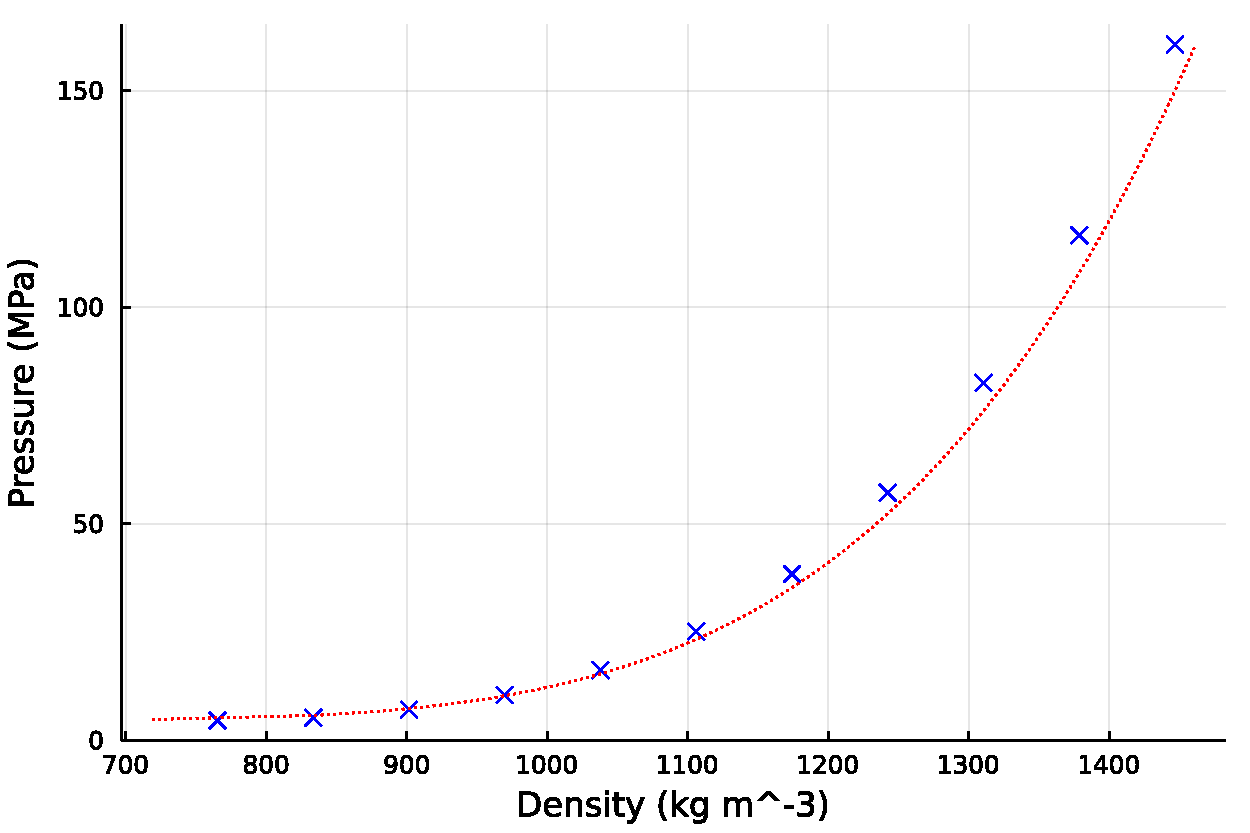
\includegraphics[width=0.7\linewidth]{figures/chapter1/argon_nvt_150K.pdf}
          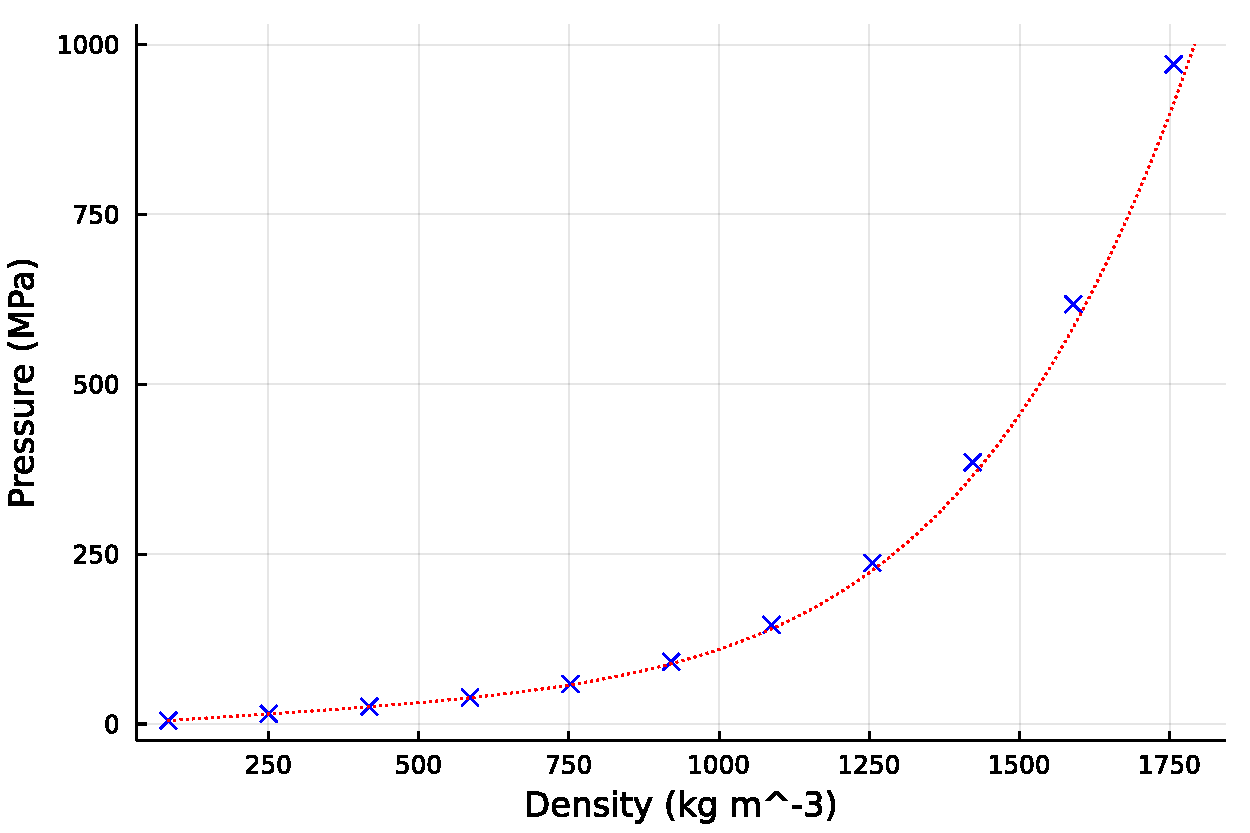
\includegraphics[width=0.7\linewidth]{figures/chapter1/argon_nvt_300K.pdf}
          \caption{ \label{fig:eos_argon}
            Simulated equations of state of Argon at 150 K (liquid phase, top) and 300 K (supercritical phase, bottom). Experimental reference curves obtained from the NIST website \cite{NIST22} are plotted in red, simulated data points correspond to blue crosses.
          }
        \end{center}
      \end{figure}

    In Figures \ref{fig:configurational_bias} and \ref{fig:kinetic_energy_bias}, we highlight the systematic error in several observables. Simulations were run for systems of $N=27$ Lennard--Jones particles, at a reduced temperature $T=1.25$ and at a reduced density $\rho=0.25$. 
    A cutoff of the potential at a distance $r_c=2.0$ was imposed, with a linear correction term ensuring that $V$ be $C^1$. 
    Additionally, regression lines were added by extrapolating the behavior at small $\Dt$ based on the theoretical expansions \eqref{eq:expansion_of_avg_in_dt}, and constraining the regression lines to converge to the same value in the limit $\Dt\to 0$.
    This was achieved by a linear least squares regression procedure.
    The result also illustrate that a possibility to reduce the systematic error is to compute a desired average for several timesteps, and computing an extrapolated value at $\Dt=0$ based on the theoretical knowledge of the behavior of the systematic error as $\Dt\to 0$. This is known as Richardson extrapolation, see for instance \cite[Section 9.6]{QSS10}.
\begin{figure}[htbp]
    \begin{center}
      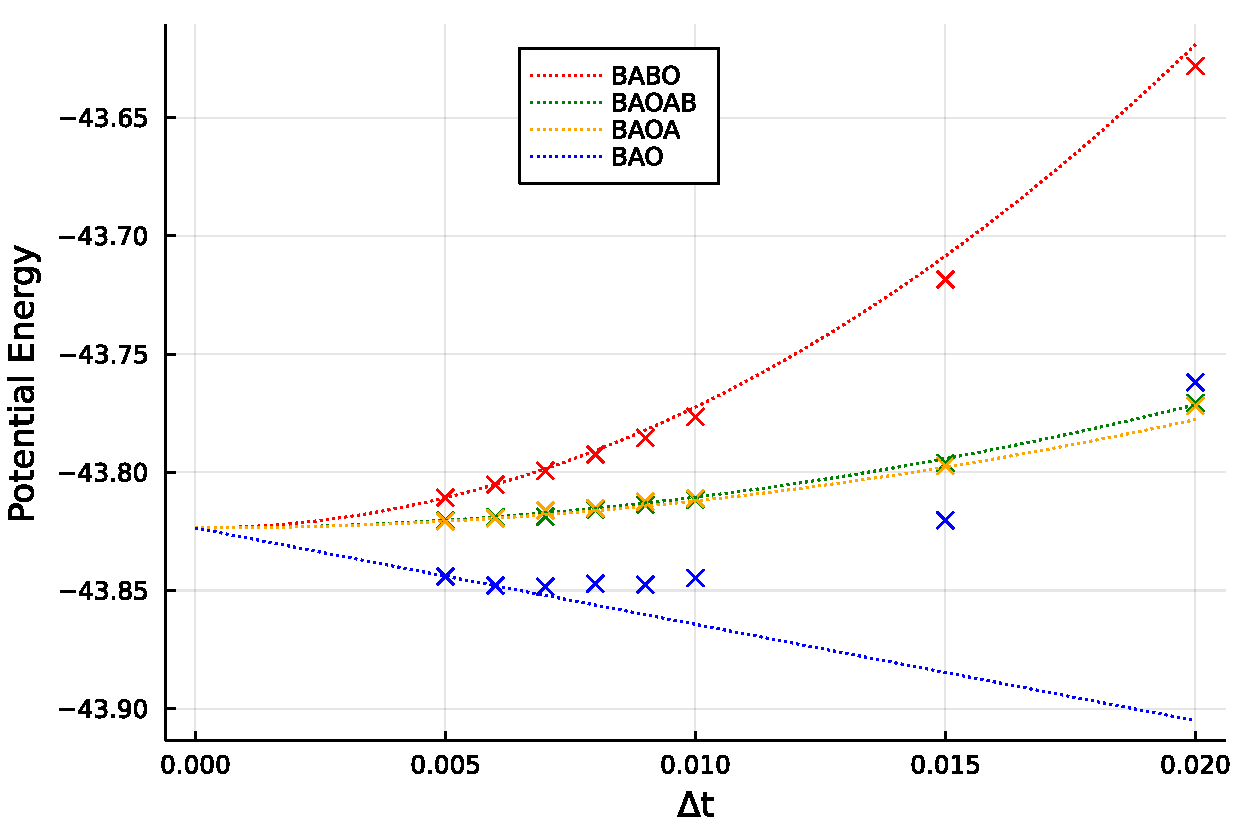
\includegraphics[width=0.49\linewidth]{figures/chapter1/potential_energy_bias.pdf}
      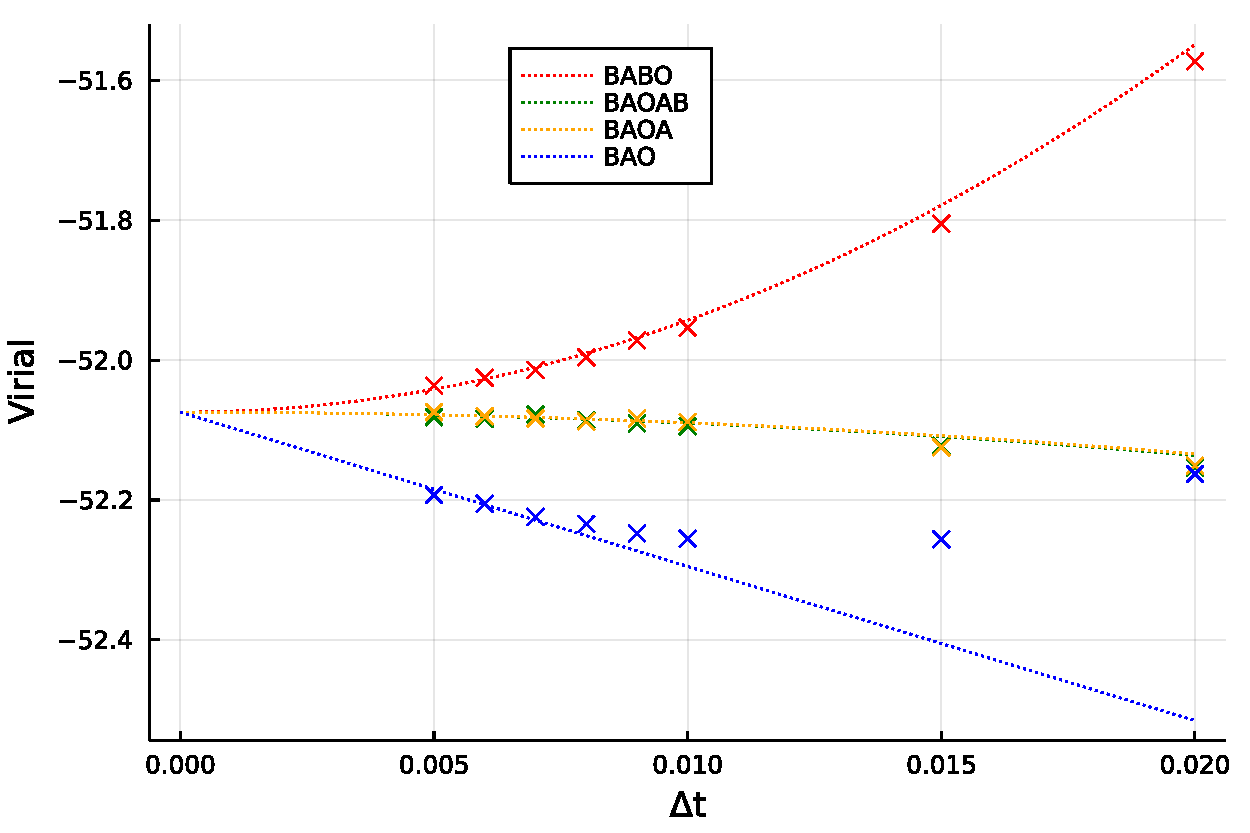
\includegraphics[width=0.49\linewidth]{figures/chapter1/virial_bias.pdf}
      \caption{ \label{fig:configurational_bias}
        Systematic error in configurational quantities for a Lennard--Jones fluid.
      }
    \end{center}
  \end{figure}

  \begin{figure}[htbp]
    \begin{center}
      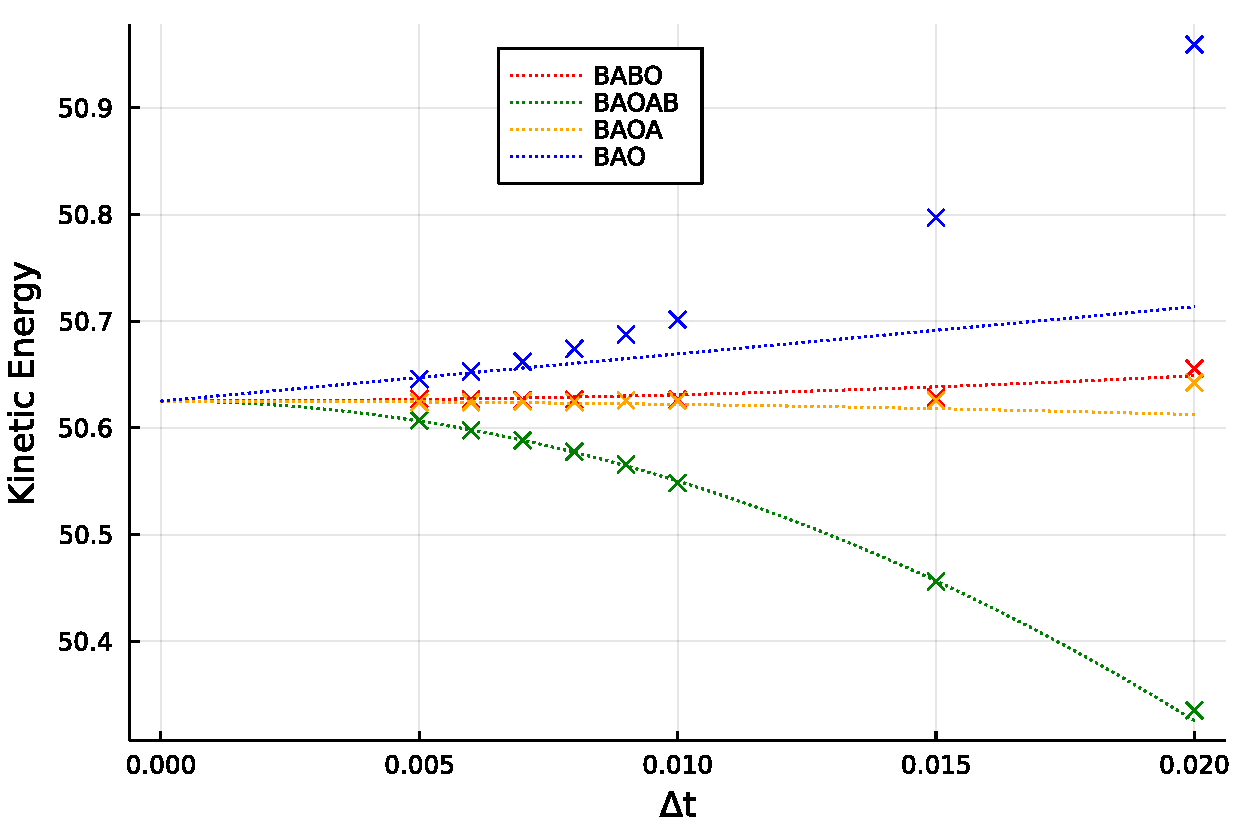
\includegraphics[width=0.7\linewidth]{figures/chapter1/kinetic_energy_bias.pdf}
      \caption{ \label{fig:kinetic_energy_bias}
        Systematic error in kinetic energy for a Lennard--Jones fluid.
      }
    \end{center}
  \end{figure}
For the two configurational quantities we investigated, the virial and potential energy, we observe an overlap in the bias between the BAOAB and BAOA schemes.
It so happens that this overlap can be simply explained by a result relating the invariant measures of certain pairs of numerical schemes, see Lemma \ref{TU_like_lemma} in the next chapter.
In fact, a preprint \cite{KK22} was recently posted, showing that a certain widely used scheme in the molecular dynamics community was equivalent to the BAOA scheme, and that the latter sampled the same configurational marginal as the BAOAB scheme.
This prompted the need for a more thorough investigation of the properties of the BAOA scheme, which we discuss in the next chapter.